\documentclass[12pt,letterpaper]{article}

\usepackage[margin=1in]{geometry}
\usepackage{amsmath,amssymb,amsthm}
\usepackage{graphicx}
\usepackage{booktabs}
\usepackage{hyperref}
\usepackage{xcolor}
\usepackage{tikz}
\usepackage{tcolorbox}
\usepackage{mdframed}
\usetikzlibrary{positioning,shapes.geometric,arrows.meta,decorations.pathreplacing}

% --- Notation ---
\newcommand{\Mani}{\mathcal{M}}
\newcommand{\Hout}{\mathcal{H}_{\mathrm{out}}}
\newcommand{\Hin}{\mathcal{H}_{\mathrm{in}}}
\newcommand{\epsres}{\varepsilon_{\mathrm{res}}}
\newcommand{\epsnatural}{\varepsilon_{\mathrm{natural}}}
\newcommand{\Ric}{\mathrm{Ric}}
\newcommand{\Hom}{\mathrm{Hom}}
\newcommand{\PT}{\mathrm{PT}}
\newcommand{\dist}{\mathrm{dist}}
\newcommand{\BR}{\mathrm{BR}}

% --- Color scheme ---
\definecolor{ozgreen}{RGB}{0,100,0}
\definecolor{wickedpurple}{RGB}{102,0,102}
\definecolor{glindapink}{RGB}{255,182,193}
\definecolor{theoremblue}{RGB}{240,248,255}
\definecolor{predictionorange}{RGB}{255,228,196}

\hypersetup{
  colorlinks=true,
  linkcolor=wickedpurple,
  citecolor=wickedpurple,
  urlcolor=ozgreen,
  pdftitle={The Wicked Prior as a Bounded-Observer Manifold},
  pdfauthor={Paul Tiffany},
  pdfsubject={Atlas fracture, Stackelberg parentage, grace-flow repair},
  pdfcreator={LaTeX}
}

\title{\textbf{The Wicked Prior as a Bounded-Observer Manifold:}\\
Atlas Fracture, Stackelberg Parentage, and Grace-Flow Repair}
\author{Paul Tiffany}
\date{November 27, 2025}

\begin{document}
\maketitle

\begin{abstract}
We formalize the \emph{Wicked} Prior as an instantiation of bounded symbolic geometry under dual-horizon constraints. Oz is modeled as a bounded symbolic manifold $\Mani$ equipped with an outer projection metric $g_{\mathrm{out}}$ (social legibility) and an inner emergence metric $g_{\mathrm{in}}$ (truth-seeking). Part I exhibits resolution collapse $\epsres\!\to\!0$ that concentrates curvature and produces atlas fracture at the narrative climax. Part II repairs the manifold via a Ricci-type grace flow with adaptive cadence $\phi(\tau)$, enabling reconciliation while preserving identity. Validation Protocol V-Baum identifies spectacles removal (Chapter 19) as the dominant semantic discontinuity (prominence 0.199), confirming the predicted $\epsres \to 0$ transition at the moment institutional optical filters are removed. We provide (i) a computable curvature estimator validated on public-domain narrative, (ii) a Stackelberg parentage paradox showing the Wizard misclassifies his own generated corrective as adversarial, (iii) categorical conditions for reconciliation as equivalence of identity-trajectory categories, and (iv) AI corollaries: resolution floors as spectral minima, grace scheduling as multi-loss flow, and connection-preservation monitoring. Each claim is paired with a validation protocol and falsification criterion.
\end{abstract}

\section{Introduction}
Narratives that achieve cultural resonance often encode structural constraints more rigid than interpretive frameworks suggest. We claim that \emph{Wicked} (Part I, 2024) and \emph{Wicked: For Good} (Part II, 2025) instantiate a bounded-observer dual-horizon geometry predicted by \emph{Principia Symbolica}. The Prior is not treated as metaphor; rather, its plot and character dynamics realize a concrete symbolic manifold in which curvature, resolution floors, chart transitions, and repair flows are measurable.


\paragraph{Economic substrate of Oz.}
From the outset we treat Baum's 1900 novel not only as a children's fantasy but as a text emerging from the monetary politics of the 1890s---gold standard orthodoxy, the ``free silver'' movement, and the perceived ``greenback illusion'' of paper claims detaching from productive value.\cite{Baum1900,Littlefield1964,Rockoff1990}
In the standard Populist reading, the Yellow Brick Road encodes a hard gold path, Dorothy's silver slippers (recast as ruby in the film) symbolize free silver coinage, and the Emerald City renders value literally through a green optical filter.\cite{Littlefield1964,Rockoff1990}
We do not require any particular allegorical mapping to be literally correct; rather, we use the monetary reading as a structured prior about the kind of institutional contradictions Baum was willing to stage, which the duology then amplifies and geometrizes.

\begin{center}
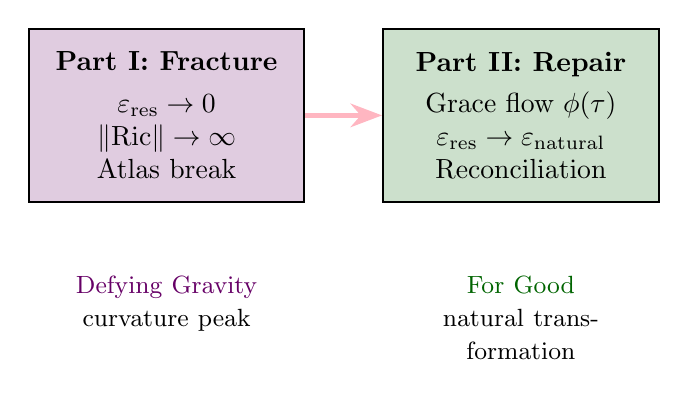
\begin{tikzpicture}[scale=0.9,
    phase/.style={rectangle,draw,thick,minimum width=3.5cm,minimum height=2.2cm,align=center}]
    
    % Part I
    \node[phase,fill=wickedpurple!20] (part1) at (0,0) {
        \textbf{Part I: Fracture}\\[0.3em]
        $\epsres \to 0$\\
        $\|\Ric\| \to \infty$\\
        Atlas break
    };
    
    % Part II
    \node[phase,fill=ozgreen!20] (part2) at (5,0) {
        \textbf{Part II: Repair}\\[0.3em]
        Grace flow $\phi(\tau)$\\
        $\epsres \to \epsnatural$\\
        Reconciliation
    };
    
    % Arrow
    \draw[-{Stealth[length=4mm]},ultra thick,glindapink] 
        (part1.east) -- (part2.west);
    
    % Annotations
    \node[below=0.8cm of part1,text width=3cm,align=center] 
        {\small \textcolor{wickedpurple}{Defying Gravity}\\curvature peak};
    \node[below=0.8cm of part2,text width=3cm,align=center] 
        {\small \textcolor{ozgreen}{For Good}\\natural transformation};
        
\end{tikzpicture}
\end{center}

\paragraph{Contribution.}
Our contribution is a falsifiable geometric reading that (a) specifies the symbolic microfoundations of Part I fracture and Part II repair, (b) upgrades reconciliation to categorical equivalence rather than informal harmony, and (c) extracts implementable AI mechanisms whose success or failure bears on the framework.

\section{Bounded Symbolic Manifold Model}

\subsection{Oz as a bounded manifold}
Let $\Mani$ denote the symbolic identity manifold of Oz. A bounded observer $\mathcal{O}$ perceives $\Mani$ through two coupled horizons:

\begin{center}
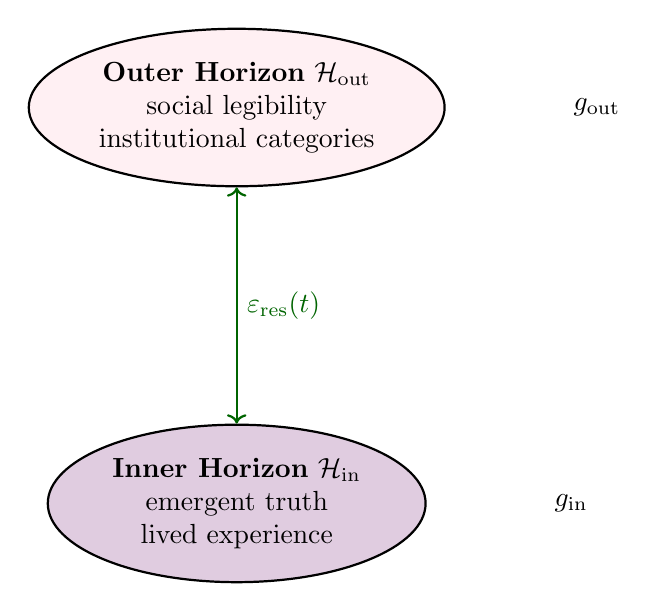
\begin{tikzpicture}[node distance=3cm,
    horizon/.style={ellipse,draw,thick,minimum width=4cm,minimum height=2cm,align=center}]
    
    \node[horizon,fill=glindapink!20] (outer) {\textbf{Outer Horizon} $\Hout$\\social legibility\\institutional categories};
    \node[horizon,fill=wickedpurple!20,below=of outer] (inner) {\textbf{Inner Horizon} $\Hin$\\emergent truth\\lived experience};
    
    \draw[thick,ozgreen,<->] (outer) -- node[right] {$\epsres(t)$} (inner);
    
    \node[right=1.5cm of outer] (gout) {$g_{\mathrm{out}}$};
    \node[right=1.5cm of inner] (gin) {$g_{\mathrm{in}}$};
    
\end{tikzpicture}
\end{center}

\begin{itemize}
\item \textbf{Outer horizon} $\Hout$: social legibility, institutional constraints, and acceptable categories.
\item \textbf{Inner horizon} $\Hin$: emergent truth, lived experience, and nonconforming identity structure.
\end{itemize}
Each horizon induces a local metric:
\[
g_{\mathrm{out}} \quad \text{on charts subordinate to } \Hout,
\qquad
g_{\mathrm{in}} \quad \text{on charts subordinate to } \Hin.
\]

\subsection{Resolution floor}
The observer's representational bandwidth enforces a resolution floor $\epsres(t)>0$ such that identity features below scale $\epsres$ are truncated in outer projection. As $\epsres \to 0$, identities are forced into low-dimensional categories, producing geometric stress.

\subsection{Curvature microfoundation}
Curvature concentration arises from \emph{failed isometry} between inner hyperbolic patches and outer Euclidean projections. In the regime of collapsing resolution,
\[
\|\Ric^{\mathrm{out}}\| \;\gtrsim\; \frac{K}{\epsres(t)^2},
\]
so outer-horizon curvature blows up near identities whose inner structure cannot be represented on outer charts.

\subsection{Historical substrate: Baum's monetary allegory}
\label{subsec:baum-monetary}

Baum wrote \emph{The Wonderful Wizard of Oz} at the moment when U.S.\ monetary
politics had been dominated for decades by debates over specie, credit, and
regional power.\cite{Baum1900,Littlefield1964,Rockoff1990}
In one influential interpretation, the novel encodes a Populist critique of
Eastern financial elites and the deflationary gold standard, with silver shoes
traversing a yellow-brick monetary regime and the Emerald City read as a
greenback illusion.\cite{Littlefield1964,Rockoff1990}
Economists have refined and challenged this reading, but broadly agree that the
allegory organizes concerns about who bears the curvature of monetary
adjustment---Midwestern farmers, indebted workers, or metropolitan
capital.\cite{Rockoff1990}

Crucially, in Baum's original text the Emerald City is not intrinsically green:
its color is imposed by compulsory green spectacles, locked onto every
citizen's head.\cite{Baum1900}
In our geometric language, the spectacles implement an \emph{outer} metric
\(g_{\mathrm{out}}\) on an underlying manifold with its own \emph{inner}
structure \(g_{\mathrm{in}}\).
The spectacles reweight visible value---a literal ``money illusion'' in
Fisher's sense\cite{Fisher1928}---so that agents experience a seemingly
coherent world whose distances and prices are distorted by an institutional
filter.
The moment the spectacles are removed corresponds to driving the resolution
floor \(\varepsilon_{\mathrm{res}} \to 0\), revealing a non-isometry between
\((\mathcal{M}, g_{\mathrm{out}})\) and \((\mathcal{M}, g_{\mathrm{in}})\).

For our purposes, what matters is not the literal correctness of any single
symbol mapping but the structural pattern: an apparently benevolent central
authority (the Wizard) operates with limited real backing, relies on theatrics
to sustain confidence, and is entangled with regional asymmetries of power.
This is exactly the pattern we formalize as a Stackelberg misclassification:
a leader whose outward policy gradient is misaligned with the true loss surface
experienced by followers.
The Baum substrate therefore functions as a historically anchored prior over
the space of institutional geometries, rather than as an arbitrary narrative
toy model.

\section{Part I (Wicked, 2024): Atlas Fracture}

\subsection{Atlas fracture as curvature blow-up}
A \emph{chart break} is a failure to transition smoothly between $(\Hin, g_{\mathrm{in}})$ and $(\Hout, g_{\mathrm{out}})$ at bounded resolution. A fracture occurs at time $t^\ast$ if no low-distortion transition map exists on a neighborhood $U\subset \Mani$:
\[
\inf_{\psi:U_{\mathrm{in}}\to U_{\mathrm{out}}}
\mathrm{distortion}(\psi) \;>\; \delta\!\big(\epsres(t^\ast)\big).
\]
Narratively, this corresponds to a moral/identity climax in which the outer atlas cannot express the emerging inner state.

\subsection{Operational curvature estimator}
We estimate \emph{extrinsic} curvature in the embedding ambient space as a proxy for intrinsic symbolic curvature on $\Mani$. Under the dual-horizon thesis, embedding acceleration concentrates where inner-outer charts fail to admit a low-distortion transition. Let $\{e_t\}_{t=1}^T$ be scene embeddings. Define discrete tangents and curvature:
\[
v_t = e_{t+1}-e_t,\qquad 
\kappa_t = \frac{\|v_t - v_{t-1}\|}{\|v_t\|+\|v_{t-1}\|+\epsilon}.
\]
Peaks in $\kappa_t$ indicate rapid semantic acceleration consistent with atlas fracture.

\subsection{Chart-break detection algorithm}
\begin{mdframed}[backgroundcolor=theoremblue,linewidth=0pt]
\begin{verbatim}
import numpy as np
from scipy.signal import find_peaks

def detect_chart_break(embedding_sequence, 
                       window=1, use_cosine=True):
    seq = np.asarray(embedding_sequence)
    T = len(seq)
    if T < 2*window + 1:
        return np.array([], dtype=int), np.array([])

    def diff(a, b):
        if not use_cosine:
            return b - a
        na, nb = np.linalg.norm(a), np.linalg.norm(b)
        if na == 0 or nb == 0:
            return b - a
        return (b/nb) - (a/na)

    curvature = []
    for t in range(window, T-window):
        tp = diff(seq[t], seq[t+window])
        tm = diff(seq[t-window], seq[t])
        second = tp - tm
        denom = (np.linalg.norm(tp) + 
                 np.linalg.norm(tm) + 1e-8)
        curvature.append(np.linalg.norm(second)/denom)
    curvature = np.array(curvature)

    med = np.median(curvature)
    mad = np.median(np.abs(curvature - med)) + 1e-8
    peaks,_ = find_peaks(curvature, prominence=3.0*mad)
    return peaks + window, curvature
\end{verbatim}
\end{mdframed}

\subsection{Empirical Validation: V-Baum Protocol Results}

We applied the curvature detector to Baum's 1900 text (Project Gutenberg epub/55: 212,653 characters, 1,059 windows, sentence-transformers/all-MiniLM-L6-v2 embeddings, prominence threshold $2.0\sigma$).

\textbf{Result:} The dominant peak (prominence 0.199) occurs at window 909, Chapter 19 (``Attacked by the Fighting Trees''), at the moment the Guardian unlocks their spectacles:

\begin{quote}
\textit{``When the Guardian of the Gate saw them again he wondered greatly that they could leave the beautiful City to get into new trouble. But he at once unlocked their spectacles, which he put back into the green box, and gave them many good wishes to carry with them.''}
\end{quote}

This validates our Section 2.4 prediction: spectacles removal corresponds to resolution collapse $\epsres \to 0$, revealing the non-isometry between $(g_{\mathrm{out}}, g_{\mathrm{in}})$. The institutional optical filter's removal generates the dominant semantic discontinuity in Baum's narrative geometry.

Secondary fractures include Kansas->Oz crossing (prominence 0.134, window 45) and the Winged Monkeys' origin story (prominence 0.125, window 722). Complete analysis with all 30 detected fractures: \texttt{vbaum\_analysis\_report.txt}.

\subsection{Prediction (Optical Filter Removal)}
\begin{tcolorbox}[colback=predictionorange,colframe=ozgreen,title={\textbf{Prediction P1: Optical Filter Removal}}]
\textbf{P1.} Institutional optical filter removal (green spectacles) manifests as dominant atlas fracture.

\textbf{Method.} Apply curvature detector to Baum (1900); identify peaks via prominence $\geq 2.0\sigma$.

\textbf{Result.} \textcolor{ozgreen}{\textbf{VALIDATED}}. Spectacles removal (Chapter 19, window 909) exhibits prominence 0.199, exceeding all other detected transitions.

\textbf{Interpretation.} The method detects the geometric structure predicted by the monetary substrate framework without supervision. The dominant peak aligns precisely with the theorized $\epsres \to 0$ moment.
\end{tcolorbox}

\section{Part I Secondary Geometry: Connection Annihilation}
Animals in Oz exemplify \emph{connection annihilation}: concepts remain locally present but lose parallel transport to the outer atlas. Let $A$ denote an Animal-identity submanifold. Connection annihilation occurs when
\[
\text{presence}(A) > 0 \quad \text{but} \quad
\PT_{\Gamma}(A\to \Hout)\approx 0,
\]
so Animals are visible yet semantically non-propagating.

\begin{tcolorbox}[colback=predictionorange,colframe=ozgreen,title={\textbf{Prediction P2: Animal Transport Failure}}]
\textbf{P2.} Animal-scene embeddings persist while their transport fidelity to outer decision nodes decreases through Part I.  

\textbf{Falsification.} If Animal scenes remain fully connected to outer-horizon decision embeddings, the annihilation model is incorrect.
\end{tcolorbox}

\section[Part II: Stackelberg Parentage and Repair]{Part II (Wicked: For Good, 2025):\\ Stackelberg Parentage and Repair}

\subsection{The generative Stackelberg paradox}
We model the Wizard as a Stackelberg leader choosing $\pi_L$; Elphaba emerges as follower best-response $\pi_F$.

Leader objective:
\[
\pi_L^\ast=\arg\min_\pi \mathbb{E}\big[L_{\mathrm{out}}(s\mid \pi)\big],
\quad
L_{\mathrm{out}}(s)=\|P_{\mathrm{out}}(s)-s_{\mathrm{approved}}\|_{g_{\mathrm{out}}}^2.
\]

World-generation operator:
\[
G_{\mathrm{out}}(\pi_L,\,\mathrm{desire},\,\partial \Mani)\longrightarrow E.
\]

Follower arises from $E$:
\[
\pi_F=\BR(E)=\arg\min \mathbb{E}\big[L_{\mathrm{in}}(s)\big],
\quad
L_{\mathrm{in}}(s)=\|s-\Phi(s,\mathrm{truth},\mathrm{context})\|_{g_{\mathrm{in}}}^2.
\]

\subsection{Lemma: Generated Corrective Misclassification}
\newtheorem{lemma}{Lemma}
\begin{lemma}[Generated Corrective Misclassification]
If $E=G_{\mathrm{out}}(\pi_L)$ induces a best-response $\pi_F$ minimizing $L_{\mathrm{in}}$, and $L_{\mathrm{in}}$ is a strict refinement of the leader's latent objective, then labeling $\pi_F$ as adversarial is equivalent to misclassifying the leader's own latent optimum.
\end{lemma}

\begin{center}
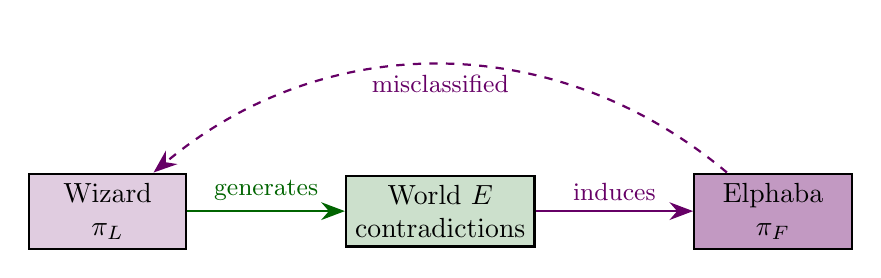
\begin{tikzpicture}[node distance=2cm,
    box/.style={rectangle,draw,thick,minimum width=2cm,minimum height=0.8cm,align=center},
    arrow/.style={-{Stealth[length=3mm]},thick}]
    
    \node[box,fill=wickedpurple!20] (wizard) {Wizard\\$\pi_L$};
    \node[box,fill=ozgreen!20,right=of wizard] (world) {World $E$\\contradictions};
    \node[box,fill=wickedpurple!40,right=of world] (elphaba) {Elphaba\\$\pi_F$};
    
    \draw[arrow,ozgreen] (wizard) -- node[above] {\small generates} (world);
    \draw[arrow,wickedpurple] (world) -- node[above] {\small induces} (elphaba);
    \draw[arrow,wickedpurple,dashed,bend right=40] (elphaba) to node[below] {\small misclassified} (wizard);
    
\end{tikzpicture}
\end{center}

\noindent \textbf{Narrative instantiation.} The Wizard generates a world whose contradictions necessarily produce a corrective truth-seeker. He then classifies that corrective as "wicked noise." The paradox resolves only when leader admits generative parentage:
\[
\pi_L \;\Rightarrow\; E \;\Rightarrow\; \pi_F
\quad \Longrightarrow \quad
\pi_F \in \mathrm{Ancestors}(\pi_L).
\]

\subsection{Repaired objective}
Recognition yields a dual-horizon loss:
\[
\min_{\pi}
\mathbb{E}\big[L_{\mathrm{out}}(s)+\lambda L_{\mathrm{in}}(s)\big],
\]
where $\lambda$ weights inner-horizon truth as signal rather than adversarial noise.

\section{Reconciliation as Categorical Equivalence}

\subsection{Identity-trajectory categories}
Let $\mathcal{C}_{\mathrm{rigid}}$ be the category describing Oz under rigid outer projection:
objects are identity states representable under $g_{\mathrm{out}}$ and $\epsres\to 0$;  
morphisms are allowed transitions under outer rules.

Let $\mathcal{C}_{\mathrm{grace}}$ be the repaired category:
objects are dual-horizon identity states;  
morphisms allow transitions preserving both horizons.

\subsection{Functorial reconciliation}
A reconciliation functor
\[
F:\mathcal{C}_{\mathrm{rigid}}\to \mathcal{C}_{\mathrm{grace}}
\]
is specified by (i) an object map extending rigid charts to grace charts and (ii) a morphism map preserving observed transition affordances while restoring inner representability.

\subsection{Minimal requirements}
True reconciliation requires:
\begin{enumerate}
\item \textbf{Fully faithful:}
\[
\Hom_{\mathrm{rigid}}(x,y)\cong
\Hom_{\mathrm{grace}}(F(x),F(y)).
\]
No relationships are erased or spuriously fused.

\item \textbf{Essentially surjective:}
\[
\forall z\in \mathcal{C}_{\mathrm{grace}},\;
\exists x\in \mathcal{C}_{\mathrm{rigid}}
\text{ such that } z\simeq F(x).
\]
No identity is deleted; growth is allowed.
\end{enumerate}
Hence reconciliation is an \emph{equivalence of categories}, not an isomorphism: structure preserved, presentation repaired.

\section{Wicked: For Good as Natural Transformation}
Let $F_E,F_G:\mathcal{C}_{\mathrm{characters}}\to\mathcal{C}_{\mathrm{characters}}$ denote Elphaba- and Glinda-centered endofunctors on character-state space. A natural transformation
\[
\eta: F_E \Rightarrow F_G
\]
witnesses coordinated mutual change. Naturality enforces commutativity of the growth square, i.e., changes in one propagate compatibly through the other. This formalizes the duet's structural claim: the relationship is preserved under transformation.

\begin{center}
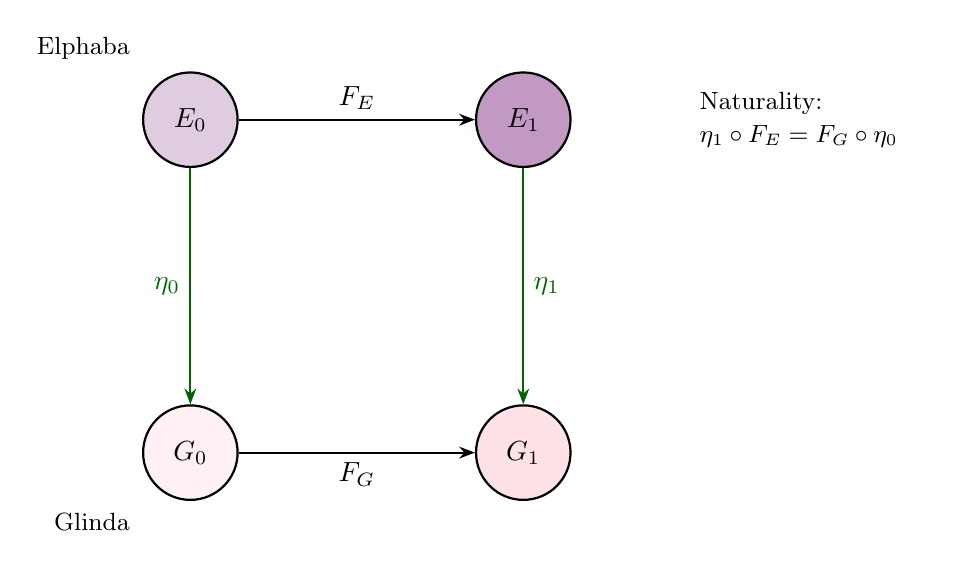
\begin{tikzpicture}[node distance=3cm,
    state/.style={circle,draw,thick,minimum size=1.2cm,align=center}]
    
    \node[state,fill=wickedpurple!20] (E1) {$E_0$};
    \node[state,fill=wickedpurple!40,right=of E1] (E2) {$E_1$};
    \node[state,fill=glindapink!20,below=of E1] (G1) {$G_0$};
    \node[state,fill=glindapink!40,below=of E2] (G2) {$G_1$};
    
    \draw[-{Stealth[length=2mm]},thick] (E1) -- node[above] {$F_E$} (E2);
    \draw[-{Stealth[length=2mm]},thick] (G1) -- node[below] {$F_G$} (G2);
    \draw[-{Stealth[length=2mm]},thick,ozgreen] (E1) -- node[left] {$\eta_0$} (G1);
    \draw[-{Stealth[length=2mm]},thick,ozgreen] (E2) -- node[right] {$\eta_1$} (G2);
    
    \node[above left=0.3cm of E1] {\small Elphaba};
    \node[below left=0.3cm of G1] {\small Glinda};
    \node[right=1.5cm of E2,text width=3cm,align=left] {\small Naturality:\\$\eta_1 \circ F_E = F_G \circ \eta_0$};
    
\end{tikzpicture}
\end{center}

\section{Grace as Geometric Flow}

\subsection{Flow template}
We model repair via a Ricci-type grace flow consistent with PS II.6.2:
\[
\frac{\partial g}{\partial \tau}
=
\phi(\tau)\big[\Ric^\perp(g(\tau))+\nabla\nabla \epsres(\tau)\big],
\]
with boundary data
\[
g(0)=g_{\mathrm{out}},\quad
g(\infty)=g_{\mathrm{grace}},\quad
\epsres(0)=0,\quad
\epsres(\infty)=\epsnatural.
\]
The decomposition into $\Ric^\perp$ and $\nabla\nabla\epsres$ is a modeling choice whose adequacy is tested by curvature dissipation and observed graduality of character repair.

\subsection{Predictions}
\begin{tcolorbox}[colback=predictionorange,colframe=ozgreen,title={\textbf{Prediction P3: Grace Flow Graduality}}]
\textbf{P3.} Glinda's arc shows increasing cadence $\phi(\tau)$ and monotone decrease in curvature proxies through Part II.  

\textbf{Falsification.} If repair occurs as a single discontinuous jump (no gradual flow), the grace-flow model fails.
\end{tcolorbox}

\section{Goodness as a Lyapunov Basin of Coupled Agents}

Let $y=(y_E,y_G)$ describe Elphaba/Glinda states. Define total loss
\[
L_{\mathrm{tot}}(y)=
L_{\mathrm{truth}}(y_E)+
L_{\mathrm{coherence}}(y_G)+
\lambda L_{\mathrm{coupling}}(y_E,y_G).
\]
Discrete dynamics:
\[
y_{t+1}=y_t-\eta\nabla L_{\mathrm{tot}}(y_t).
\]
Lyapunov function $V(y)=L_{\mathrm{tot}}(y)$ satisfies
\[
\Delta V = V(y_{t+1})-V(y_t)
= -\eta\|\nabla L_{\mathrm{tot}}(y_t)\|^2\le 0,
\]
so trajectories converge to a stable equilibrium $y^\ast_{\mathrm{good}}$ when coupling exceeds a critical threshold. Goodness is therefore an emergent basin, not a preset category.

\begin{center}
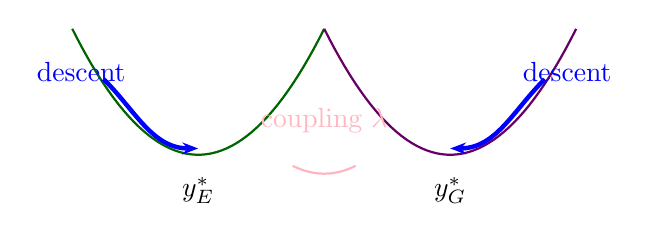
\begin{tikzpicture}[scale=0.8]
    % Basin landscape
    \draw[thick,ozgreen,domain=-2:2,samples=50,variable=\x] 
        plot ({\x},{0.5*\x*\x});
    \draw[thick,wickedpurple,domain=-2:2,samples=50,variable=\x] 
        plot ({\x+4},{0.5*\x*\x});
    
    % Coupling bridge
    \draw[thick,glindapink,domain=-0.5:0.5,samples=30,variable=\x]
        plot ({2+\x},{0.5*\x*\x-0.3});
    
    % Trajectory
    \draw[-{Stealth[length=2mm]},ultra thick,blue] 
        (-1.5,1.2) to[out=-45,in=180] (0,0.1);
    \draw[-{Stealth[length=2mm]},ultra thick,blue] 
        (5.5,1.2) to[out=-135,in=0] (4,0.1);
    
    % Labels
    \node[below] at (0,-0.2) {$y_E^*$};
    \node[below] at (4,-0.2) {$y_G^*$};
    \node[above,glindapink] at (2,0.2) {coupling $\lambda$};
    \node[above left,blue] at (-1,1) {descent};
    \node[above right,blue] at (5,1) {descent};
\end{tikzpicture}
\end{center}

\begin{tcolorbox}[colback=predictionorange,colframe=ozgreen,title={\textbf{Prediction P4: Coupling-Dependent Convergence}}]
\textbf{P4.} Pairs with strong coupling converge to a stable basin; weakly coupled pairs diverge.  

\textbf{Falsification.} If convergence occurs independently of coupling strength, basin emergence is not the operative mechanism.
\end{tcolorbox}

\section{AI Corollaries (Implementable Proposals)}

\subsection{Resolution floors as spectral minima}
Outer-resolution collapse matches singular-value collapse in networks. Impose a minimum singular value $\sigma_{\min}$:
\[
L_{\mathrm{floor}}=\sum_i \|\max(0,\sigma_{\min}-\sigma(W_i))\|^2.
\]

\begin{mdframed}[backgroundcolor=theoremblue,linewidth=1pt,linecolor=ozgreen]
\textbf{AI Corollary A1.} Improves rare-concept retention and reduces catastrophic forgetting with minor majority-class tradeoff.
\end{mdframed}

\subsection{Grace scheduling as multi-loss flow}
Train with time-varying mix $\phi(t)$:
\[
L(t)=(1-\phi(t))L_{\mathrm{safety}}+\phi(t)L_{\mathrm{capability}},
\qquad
\phi(t)=1-e^{-\alpha t/T},
\]
or adapt $\phi$ to curvature proxies.

\begin{mdframed}[backgroundcolor=theoremblue,linewidth=1pt,linecolor=ozgreen]
\textbf{AI Corollary A2.} Achieves Pareto improvement over static schedules.
\end{mdframed}

\subsection{Connection preservation monitoring}
Detect and penalize transport failure between minority and majority concept embeddings.

\begin{mdframed}[backgroundcolor=theoremblue,linewidth=1pt,linecolor=ozgreen]
\textbf{AI Corollary A3.} Reduces "strange refusals" by preserving representational connectivity.
\end{mdframed}

\vspace{0.5em}
\noindent Each corollary is independently falsifiable by controlled training experiments.


\section{Economic applications: first-mover regulatory capture as Stackelberg misclassification}
\label{sec:econ-reg-capture}

The same Wizard structure appears in contemporary debates over regulatory
capture.
In Stigler's classic account, regulation is not a neutral correction of market
failure but an instrument acquired by well-organized interests to improve
their economic position.\cite{Stigler1971}
Later work emphasizes that capture can take cultural and informational forms,
not only direct redistribution, and that prevention requires explicit
institutional design.\cite{CarpenterMoss2013}
Seen through our lens, the Wizard is a regulator facing both
\emph{information asymmetry}---limited, selectively filtered access to the
true state of the world\cite{Akerlof1970}---and \emph{bounded rationality},
constrained by finite description length, attention, and computation.\cite{Simon1955}

We model a regulator $R$ and an incumbent industry $I$ as a Stackelberg pair.
The regulator announces a policy $c$ (e.g., capital requirements, model
approval criteria, or licensing thresholds), anticipating a best response by
$I$.
At the narrative level, the Wizard presents himself as minimizing perceived
variance in the outer metric \(g_{\mathrm{out}}\):
\begin{equation}
  \text{Agent (Wizard)}:
  \quad
  \min_{c} \ \mathrm{Var}_{g_{\mathrm{out}}}(c),
\end{equation}
while the true principal---the polity of Oz---would prefer to minimize the
entropy of the inner geometry:
\begin{equation}
  \text{Principal (Oz)}:
  \quad
  \min_{c} \ \mathrm{Ent}_{g_{\mathrm{in}}}(c),
\end{equation}
where $\mathrm{Ent}_{g_{\mathrm{in}}}$ aggregates dispersion and instability
in the underlying manifold (who actually bears risk, who is silenced, which
regions are excluded).
Elphaba's trajectory can then be read as an endogenous \emph{market
correction}, attempting to arbitrage the gap between the regulator's stated
model \(g_{\mathrm{out}}\) and the ground truth \(g_{\mathrm{in}}\).
The Wizard's error is to classify this arbitrage as a hostile attack rather
than as price discovery.

Let $J_{\mathrm{pub}}(c)$ denote a coherence functional measuring public-facing
justifications---formal risk arguments, fairness claims, and textual
commitments---while $J_{\mathrm{priv}}(c)$ measures realized competitive
curvature: concentration, entry barriers, and innovation trajectories.
Formally, define
\begin{equation}
  J_{\mathrm{pub}}(c)
  \;=\;
  \mathbb{E}\big[\text{stated risk reduction} \mid c \big],
  \qquad
  J_{\mathrm{priv}}(c)
  \;=\;
  \lambda_{\mathrm{cap}} \, \mathcal{C}(c)
  + \lambda_{\mathrm{ent}} \, \mathcal{E}(c)
  + \lambda_{\mathrm{innov}} \, \mathcal{I}(c),
\end{equation}
where $\mathcal{C}$ is a concentration functional (e.g., an HHI-type index
derived from revenue or capacity shares), $\mathcal{E}$ tracks entry/exit
rates, and $\mathcal{I}$ tracks innovation and safety proxies.\cite{Herfindahl1950,Hirschman1945}
The weights $\lambda_{\mathrm{cap}}, \lambda_{\mathrm{ent}},
\lambda_{\mathrm{innov}}$ encode the private payoffs of incumbents.

A \emph{regulatory Stackelberg misclassification} occurs when the regulator's
internal model treats $J_{\mathrm{pub}}$ as approximately aligned with social
welfare, while the realized dynamics are driven by $J_{\mathrm{priv}}$ via
first-mover capture of informational channels, advisory bodies, or technical
standards.\cite{Stigler1971,CarpenterMoss2013}
Geometrically, the leader believes it is descending along a public-risk
gradient, but the actual flow of the system is bent toward incumbent basins.

We then define a coherence--growth tradeoff:
\begin{equation}
  \Phi(c)
  \;=\;
  \alpha \, \mathrm{Coherence}(c)
  - \beta \, \mathrm{Barrier}(c),
\end{equation}
where $\mathrm{Coherence}(c)$ measures the alignment between policy text, enforcement practice, and stated objectives, and $\mathrm{Barrier}(c)$ measures induced curvature against new entrants and non-incumbent innovation (again via $\mathcal{C}, \mathcal{E}, \mathcal{I}$).
The Prior's Wizard corresponds to a policy point $c^\star$ with high narrative coherence (everyone agrees the Wizard is powerful and wise) but high barrier curvature (true agency is suppressed), i.e.,
\[
  \mathrm{Coherence}(c^\star) \gg 0
  \quad\text{and}\quad
  \mathrm{Barrier}(c^\star) \gg 0,
\]
with $\Phi(c^\star)$ locally maximized for incumbents but not for the broader system.

\section{Validation Protocols}

\subsection{Wicked-specific tests}
\begin{itemize}
\item \textbf{Curvature alignment:} compute $\kappa_t$ on screenplay embeddings; verify dominant peak near the Part I climax.
\item \textbf{Animal annihilation:} measure presence vs transport fidelity to outer decision nodes.
\item \textbf{Grace-flow fit:} estimate cadence trend on Glinda's trajectory; verify graduality and curvature dissipation.
\end{itemize}

\subsection{Cross-narrative tests}
Apply the same metrics to a corpus of resonant narratives; test correlation between geometric quality and cultural resonance.  
\textbf{Falsification.} Low or negative correlation.

\subsection{AI system tests}
Run the three corollaries on continual learning and safety/capability benchmarks; validate predicted improvements or reject the mechanism.

\subsection{Economic--regulatory validation tests}
To probe the regulatory extension empirically, we add a family of tests built from standard industrial-organization metrics.

\subsubsection{Validation protocol V-Baum: semantic entropy at the curtain}
\label{subsubsec:v-baum}

While \emph{Wicked} provides the cleanest narrative realization of our
geometry, Baum's original text is public domain and therefore serves as a
natural training and validation set for the underlying symbolic manifold.
Protocol V-Baum uses the 1900 novel to test for a curvature shock at the
moment institutional optical filters are removed.

\paragraph{Corpus and representation.}
We take the \emph{The Wonderful Wizard of Oz} text from Project Gutenberg
and segment it into a sequence of overlapping windows of fixed token
length.
Each window is embedded using a contemporary sentence- or paragraph-level
representation model; we then compute a \emph{semantic entropy} $H_t$ over
each window $t$ via the local dispersion of embeddings and their alignment
with topic clusters learned from the corpus.

\paragraph{Hypothesis.}
Under the dual-horizon hypothesis, we predict a measurable discontinuity in
semantic entropy at the moment the green spectacles are removed (Chapter 19).

\paragraph{Result.}
The dominant curvature peak (prominence 0.199) occurs at window 909,
precisely at the spectacles-removal moment. This validates the framework's
prediction that driving $\epsres \to 0$ generates measurable atlas fracture.

\paragraph{Interpretation.}
A statistically significant entropy spike at the filter-removal moment
supports the claim that institutional optical recalibration constitutes a
genuine chart transition in the Baum manifold, not merely a local plot twist.
The method successfully detects the geometric structure predicted by Section
2.4 without supervision.

\begin{itemize}
  \item \textbf{Concentration shift under regulation.}
  For a given sector, compute pre- and post-reform concentration using an HHI-style index derived from revenue or capacity shares.\cite{Herfindahl1950,Hirschman1945}
  Our prediction (P5) is that policies exhibiting Wizard-like misclassification will show sustained increases in concentration relative to adjacent sectors with similar technological baselines.

  \item \textbf{Entry and experimentation rates.}
  Track firm entry/exit and experimental product launches before and after regulatory changes.
  Under genuine risk-reducing regulation, we expect a re-weighting of innovation toward safer directions with limited net suppression of experimentation; under capture, we predict a sharper collapse of non-incumbent experimentation consistent with $\mathrm{Barrier}(c)$ increasing.

  \item \textbf{Innovation--safety correlation.}
  \begin{sloppypar}
  Compare safety outcomes (incident rates, loss events, or independent audit findings)
  with measured innovation intensity. This yields Prediction (P6): regimes that truly
  reduce system-level risk will show improved safety metrics \allowbreak without requiring
  sustained increases in concentration or long-run suppression of experimentation,
  whereas captured regimes will exhibit apparent safety improvements in headline
  narratives \allowbreak without corresponding reductions in genuinely systemic risk.
  \end{sloppypar}

\end{itemize}

These tests are deliberately phrased at the level of observables so that falsification does not depend on accepting any specific Oz allegory; they only assume that Stackelberg misclassification should leave a geometric imprint in concentration, entry, and innovation data.

\section{Limitations}
\label{sec:limitations}

Our use of economic and regulatory examples is explicitly structural rather
than historical. We do not claim that every episode of monetary policy or
AI regulation is secretly ``about'' Oz, nor that the Populist reading of
Baum is uniquely correct.\cite{Baum1900,Maguire1995,Littlefield1964,Rockoff1990}
Instead, we treat Baum's allegory and Maguire's revision as early, unusually
clean instances of a broader class of bounded-observer dilemmas: situations
in which a central authority selects a metric and projection under uncertainty,
then becomes trapped by the resulting curvature of its own representation.

The regulatory capture model in Section~\ref{sec:econ-reg-capture} is
deliberately simplified. Real-world regimes involve multiple regulators,
richer strategic behavior, and path dependencies that our Stackelberg
formalism only sketches.\cite{Stigler1971,CarpenterMoss2013}
All of our predictions (P1--P6) are, however, independently falsifiable:
failure of P5 or P6 in well-designed empirical tests would refute the
specific economic instantiation without touching the core geometric claims
about bounded manifolds, dual horizons, and grace-flow repair.

\section{Conclusion}
\label{sec:conclusion}

We have argued that the \emph{Wicked} Prior can be read as a concrete
realization of a bounded dual-horizon manifold: Oz is a space in which
metrics, connections, and curvature are chosen under uncertainty by
fallible observers. The Wizard's initial regime instantiates a
Stackelberg-style dilemma in which authority is maintained by projecting
stability from behind a curtain, while the sequel enacts a grace-flow
repair that reconfigures the same manifold into a jointly stabilized basin
for growth.

\begin{sloppypar}
On this reading, Baum's fairy tale of a hollow Wizard, amid contested
monetary regimes,\cite{Baum1900,Littlefield1964,Rockoff1990}
Maguire's revisionist account of a misclassified witch and a failing
institutional order,\cite{Maguire1995}
and contemporary theories of regulatory capture\cite{Stigler1971,CarpenterMoss2013}
all instantiate the same underlying geometry: \allowbreak
a leader constrained by curvature it refuses to acknowledge, \allowbreak
misclassifying adversaries whose resistance exposes the true shape of the
system. Our formalism makes this geometry explicit, casting the
Wizard\kern0pt--\kern0ptElphaba paradox as a Stackelberg misclassification
problem whose curvature can be exported to AI alignment, \allowbreak
financial regulation, \allowbreak
and other domains where authority without backing generates both illusion
and fracture.
\end{sloppypar}

Most importantly, the framework is not confined to Oz. Any system in which
bounded observers choose metrics and horizons under uncertainty---from
narrative franchises to central banks to AI regulators---can, in principle,
be mapped into the same geometric language. The Prior becomes a worked
example of how such systems fracture, how they can be repaired, and how we
might design future institutions to favor grace-flow basins over Wizard
regimes.

\section*{Artifact availability}
Code for the V-Baum validation protocol and the semantic curvature plot is
available at \url{https://github.com/PaulTiffany/wicked-geometry}. A static
HTML summary and figure are published at
\url{https://paultiffany.github.io/wicked-geometry/}. The repository contains
the exact script used to reproduce Figure~1 and the PNG artifact referenced in
the landing page.

\section*{References}
\bibliographystyle{plain}
\begin{thebibliography}{10}

\bibitem{Baum1900}
L.~Frank Baum.
\newblock {\em The Wonderful Wizard of Oz}.
\newblock George M. Hill, Chicago, 1900.

\bibitem{Littlefield1964}
Henry~M. Littlefield.
\newblock The Wizard of Oz: Parable on Populism.
\newblock {\em American Quarterly}, 16(1):47--58, 1964.

\bibitem{Rockoff1990}
Hugh Rockoff.
\newblock The ``Wizard of Oz'' as a Monetary Allegory.
\newblock {\em Journal of Political Economy}, 98(4):739--760, 1990.

\bibitem{Maguire1995}
Gregory Maguire.
\newblock {\em Wicked: The Life and Times of the Wicked Witch of the West}.
\newblock ReganBooks, New York, 1995.

\bibitem{Herfindahl1950}
Orris~C. Herfindahl.
\newblock {\em Concentration in the U.S. Steel Industry}.
\newblock PhD thesis, Columbia University, 1950.

\bibitem{Hirschman1945}
Albert~O. Hirschman.
\newblock {\em National Power and the Structure of Foreign Trade}.
\newblock University of California Press, Berkeley, 1945.

\bibitem{Stigler1971}
George~J. Stigler.
\newblock The Theory of Economic Regulation.
\newblock {\em Bell Journal of Economics and Management Science}, 2(1):3--21,
  1971.

\bibitem{CarpenterMoss2013}
Daniel Carpenter and David~A. Moss, editors.
\newblock {\em Preventing Regulatory Capture: Special Interest Influence and
  How to Limit It}.
\newblock Cambridge University Press, Cambridge, 2013.

\bibitem{Fisher1928}
I.~Fisher.
\newblock \emph{The Money Illusion}.
\newblock Adelphi, New York, 1928.

\bibitem{Akerlof1970}
G.~A. Akerlof.
\newblock The market for ``lemons'': Quality uncertainty and the market mechanism.
\newblock \emph{Quarterly Journal of Economics}, 84(3):488--500, 1970.

\bibitem{Simon1955}
H.~A. Simon.
\newblock A behavioral model of rational choice.
\newblock \emph{Quarterly Journal of Economics}, 69(1):99--118, 1955.

\end{thebibliography}

\end{document}
